\documentclass[10pt]{beamer}
\usetheme{Combo}
\usepackage[utf8]{inputenc}
\usepackage[english]{babel}
\usepackage{graphicx}
\usepackage{tikz}
\usepackage{amsmath}
\usetikzlibrary{shapes,arrows,positioning}
\author{Giovanni Bacci}
\title{Mining Microbiomes}
\subtitle{Computational Biology approaches to uncover the complexity of bacterial communities}
\institute{University of Florence\\
CRA-RPS}
\date{February 10, 2015}
%\setbeamercovered{transparent} 
%\setbeamertemplate{navigation symbols}{} 
%\logo{} 
%\date{} 
%\subject{} 
\begin{document}

\begin{frame}[plain]
\titlepage
\end{frame}

%%%%%%%%%%%%%%%%%%%%%%%%%%%%%%%%%%%%%%%%%%%%%%%%%%%%%%%%%%%%%%%%%%%%%%%%%%%%%%%%%%%%%%%%%%%%%%%%%%%%%%%%%%%%%%%%%%%%%%%%%%%%%%%%%%%
%%% START - BACKGROUND
%%%%%%%%%%%%%%%%%%%%%%%%%%%%%%%%%%%%%%%%%%%%%%%%%%%%%%%%%%%%%%%%%%%%%%%%%%%%%%%%%%%%%%%%%%%%%%%%%%%%%%%%%%%%%%%%%%%%%%%%%%%%%%%%%%%
\section{Background}
\subsection{}

%%%%%%%%%%%%%%%%%%%%%%%%%%%%%%%%%%%%%%%%%%%%%%%%%%%%%%%%%%%%%%%%%%%%%%%%%%%%%%%%%%%%%%%%%%%%%%%%%%%%%%%%%%%%%%%%%%%%%%%%%%%%%%%%%%%
%%% START - Slide 1 
%%%%%%%%%%%%%%%%%%%%%%%%%%%%%%%%%%%%%%%%%%%%%%%%%%%%%%%%%%%%%%%%%%%%%%%%%%%%%%%%%%%%%%%%%%%%%%%%%%%%%%%%%%%%%%%%%%%%%%%%%%%%%%%%%%%
\begin{frame}
\vspace{4mm}
\begin{center}
	{\Large\textbf{A bacterial World...}}
\end{center}
\vspace{-2mm}
		\begin{center}
			\begin{overlayarea}{1\textwidth}{0.2\textheight}
			\only<1>{
			\begin{block}{}
				\begin{center}
					Bacteria are often cited as examples of one of the Earth’s most primitive living forms		
				\end{center}
			\end{block}
			}
			\only<2>{
			\begin{block}{}
				\begin{center}
					They have been always considered from an anthropocentric perspective
				\end{center}
			\end{block}
			}
			\only<3>{
			\begin{block}{}
				\begin{center}
					They are still associated almost exclusively to infection diseases
				\end{center}
			\end{block}
			}
			\only<4>{
			\begin{block}{}
				\begin{center}
					They are often studied to develop new antibiotic treatments
				\end{center}
			\end{block}
			}
			\only<5>{
			\begin{block}{}
				\begin{center}
					But reality is rather different
				\end{center}
			\end{block}
			}
			\only<6>{
			\begin{block}{}
				\begin{center}
					Only a very small fraction of bacteria is able to cause infections
				\end{center}
			\end{block}
			}
			\only<7>{
			\begin{block}{}
				\begin{center}
					A highly diversified and beneficial bacterial world exists
				\end{center}
			\end{block}
			}
			\end{overlayarea}
		\end{center}
		\begin{center}
			\begin{overlayarea}{1\textwidth}{0.6\textheight}
			\only<1>{\begin{center}
\includegraphics[width=0.8\textwidth]{./images/bacwcartoon/bacterial_world1-01}\end{center}}
			\only<2>{\begin{center}
\includegraphics[width=0.8\textwidth]{./images/bacwcartoon/bacterial_world2-01}\end{center}}
			\only<3>{\begin{center}
\includegraphics[width=0.8\textwidth]{./images/bacwcartoon/bacterial_world3-01}\end{center}}
			\only<4>{\begin{center}
\includegraphics[width=0.8\textwidth]{./images/bacwcartoon/bacterial_world4-01}\end{center}}
			\only<5>{\begin{center}
\includegraphics[width=0.8\textwidth]{./images/bacwcartoon/bacterial_world5-01}\end{center}}
			\only<6>{\begin{center}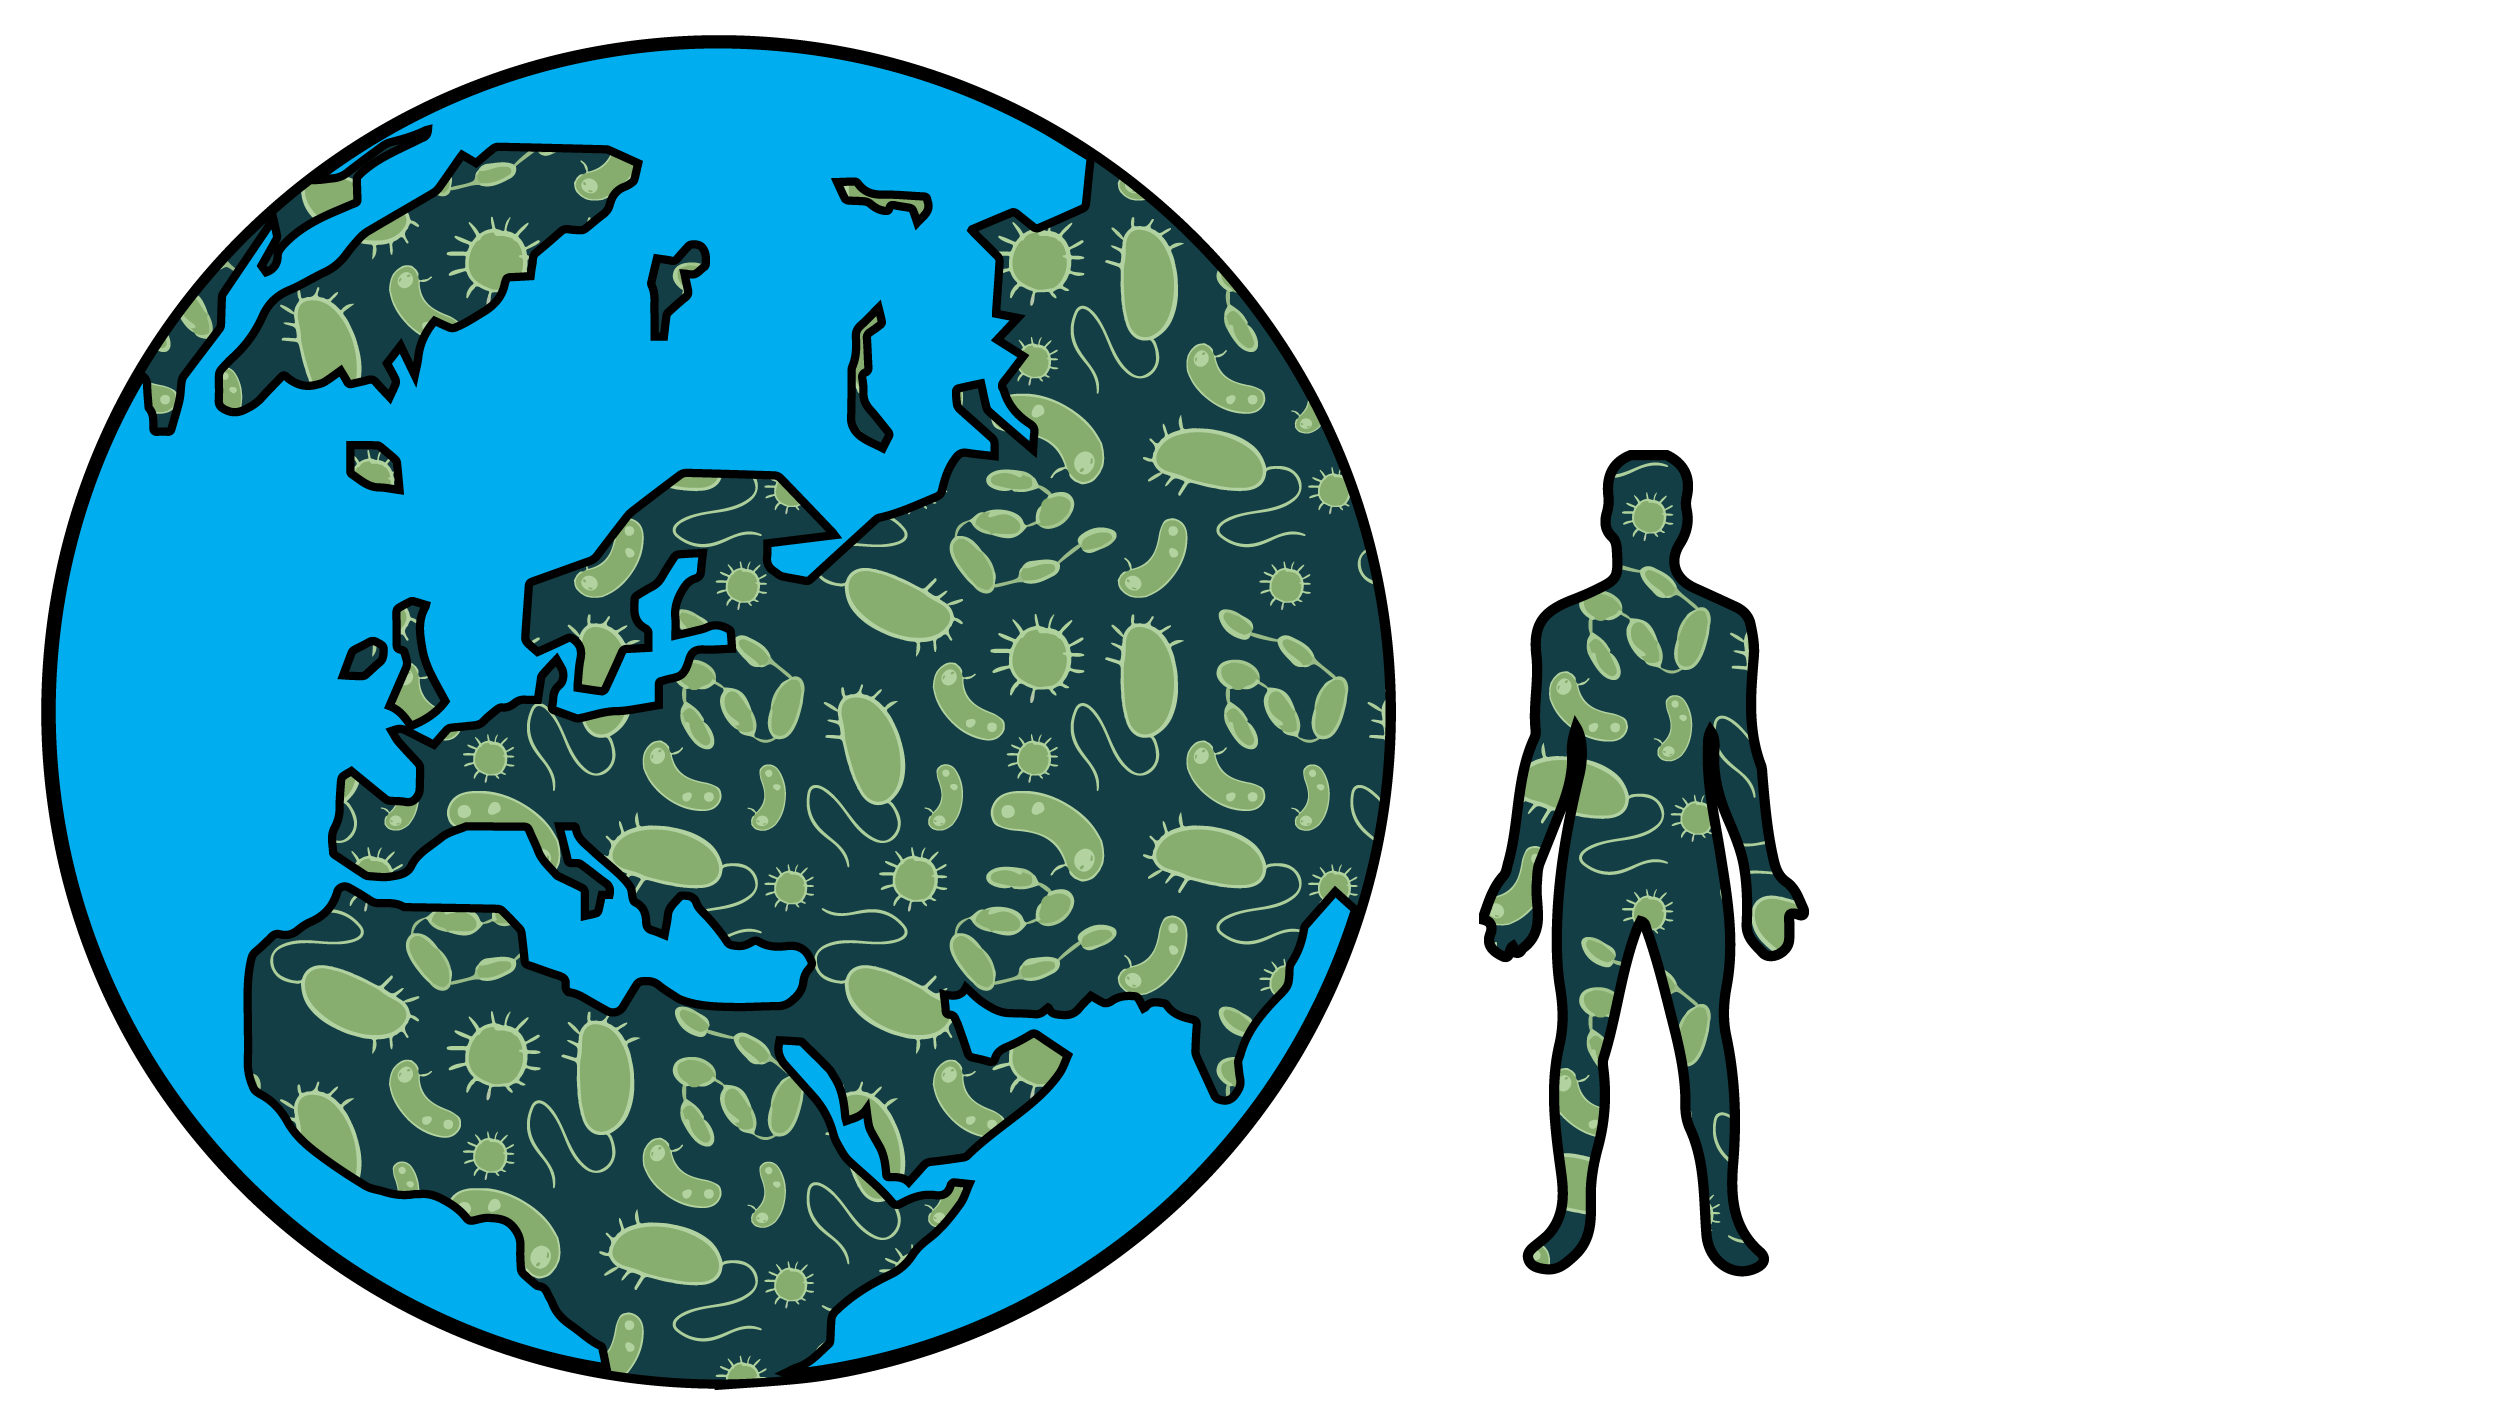
\includegraphics[width=0.8\textwidth]{./images/bacwcartoon/bacterial_world6-01}\end{center}}
			\only<7>{\begin{center}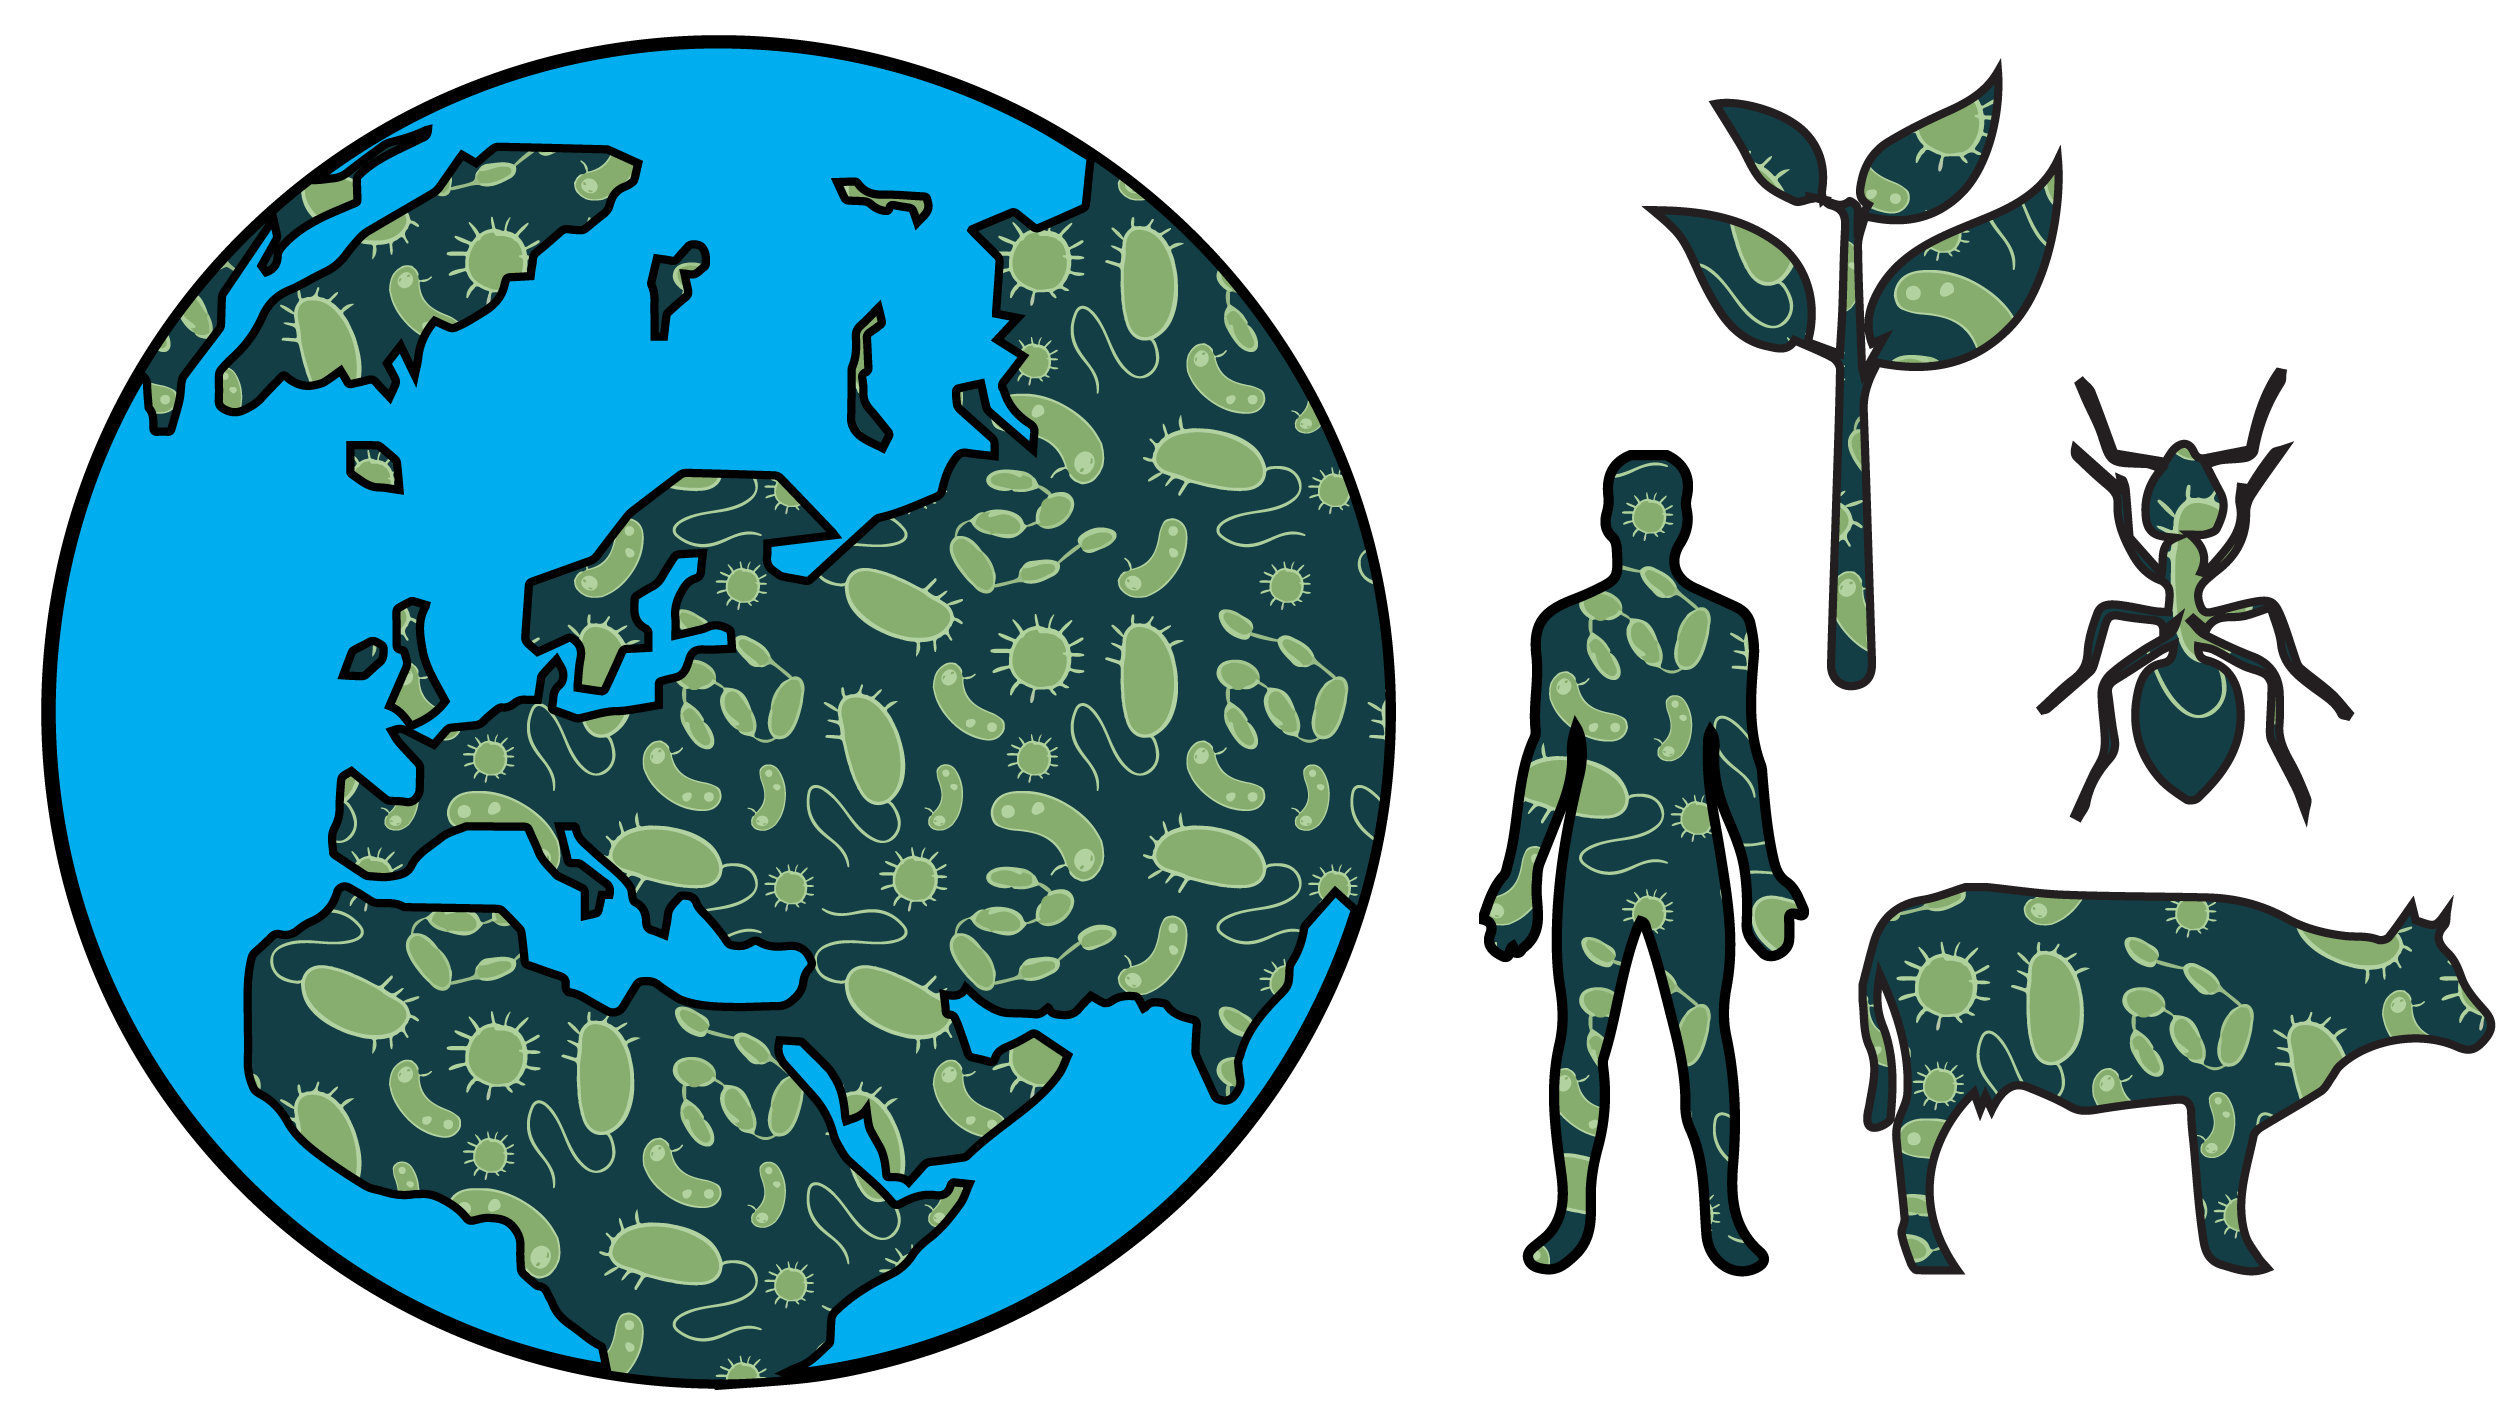
\includegraphics[width=0.8\textwidth]{./images/bacwcartoon/bacterial_world7-01}\end{center}}	
			\end{overlayarea}		
		\end{center}
\end{frame}
%%%%%%%%%%%%%%%%%%%%%%%%%%%%%%%%%%%%%%%%%%%%%%%%%%%%%%%%%%%%%%%%%%%%%%%%%%%%%%%%%%%%%%%%%%%%%%%%%%%%%%%%%%%%%%%%%%%%%%%%%%%%%%%%%%%
%%% END - Slide 1 
%%%%%%%%%%%%%%%%%%%%%%%%%%%%%%%%%%%%%%%%%%%%%%%%%%%%%%%%%%%%%%%%%%%%%%%%%%%%%%%%%%%%%%%%%%%%%%%%%%%%%%%%%%%%%%%%%%%%%%%%%%%%%%%%%%%

%%%%%%%%%%%%%%%%%%%%%%%%%%%%%%%%%%%%%%%%%%%%%%%%%%%%%%%%%%%%%%%%%%%%%%%%%%%%%%%%%%%%%%%%%%%%%%%%%%%%%%%%%%%%%%%%%%%%%%%%%%%%%%%%%%%
%%% START - Slide 2
%%%%%%%%%%%%%%%%%%%%%%%%%%%%%%%%%%%%%%%%%%%%%%%%%%%%%%%%%%%%%%%%%%%%%%%%%%%%%%%%%%%%%%%%%%%%%%%%%%%%%%%%%%%%%%%%%%%%%%%%%%%%%%%%%%%
\begin{frame}
	\begin{overlayarea}{1\textwidth}{0.9\textheight}
	\only<1>{\begin{center}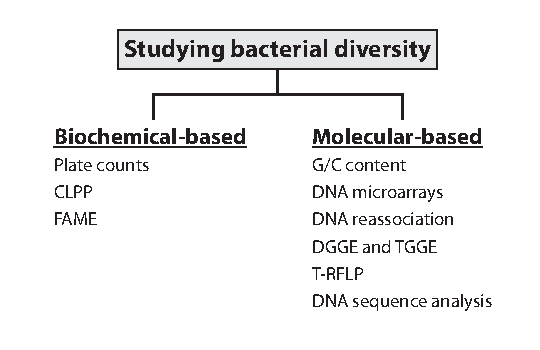
\includegraphics[width=0.7\textwidth]{./images/diversity/div-1.eps}\end{center}}
	\only<2>{\begin{center}
\includegraphics[width=0.7\textwidth]{./images/diversity/div-2.eps}\end{center}}
	\only<3->{\begin{center}
\includegraphics[width=0.7\textwidth]{./images/diversity/div-3.eps}\end{center}}
	\vspace{-2mm}
	\only<4->{
	\begin{block}{}	
	\begin{center}
		\textit{Metagenomics (also referred to as environmental and community genomics) is the genomic analysis of microorganisms by direct extraction and cloning of DNA from an assemblage of microorganisms.}\\
		\hfill\cite{handelsman2004metagenomics}
	\end{center}		
	\end{block}
	}
	\end{overlayarea}
\end{frame}
%%%%%%%%%%%%%%%%%%%%%%%%%%%%%%%%%%%%%%%%%%%%%%%%%%%%%%%%%%%%%%%%%%%%%%%%%%%%%%%%%%%%%%%%%%%%%%%%%%%%%%%%%%%%%%%%%%%%%%%%%%%%%%%%%%%
%%% END - Slide 2
%%%%%%%%%%%%%%%%%%%%%%%%%%%%%%%%%%%%%%%%%%%%%%%%%%%%%%%%%%%%%%%%%%%%%%%%%%%%%%%%%%%%%%%%%%%%%%%%%%%%%%%%%%%%%%%%%%%%%%%%%%%%%%%%%%%

%%%%%%%%%%%%%%%%%%%%%%%%%%%%%%%%%%%%%%%%%%%%%%%%%%%%%%%%%%%%%%%%%%%%%%%%%%%%%%%%%%%%%%%%%%%%%%%%%%%%%%%%%%%%%%%%%%%%%%%%%%%%%%%%%%%
%%% START - Slide 3
%%%%%%%%%%%%%%%%%%%%%%%%%%%%%%%%%%%%%%%%%%%%%%%%%%%%%%%%%%%%%%%%%%%%%%%%%%%%%%%%%%%%%%%%%%%%%%%%%%%%%%%%%%%%%%%%%%%%%%%%%%%%%%%%%%%
\begin{frame}
	\begin{columns}
		
		\begin{column}{0.5\textwidth}
			\vspace{-2mm}
			\begin{center}
				\Large\textbf{Great plate count anomaly}	
			\end{center}
			\begin{center}			
			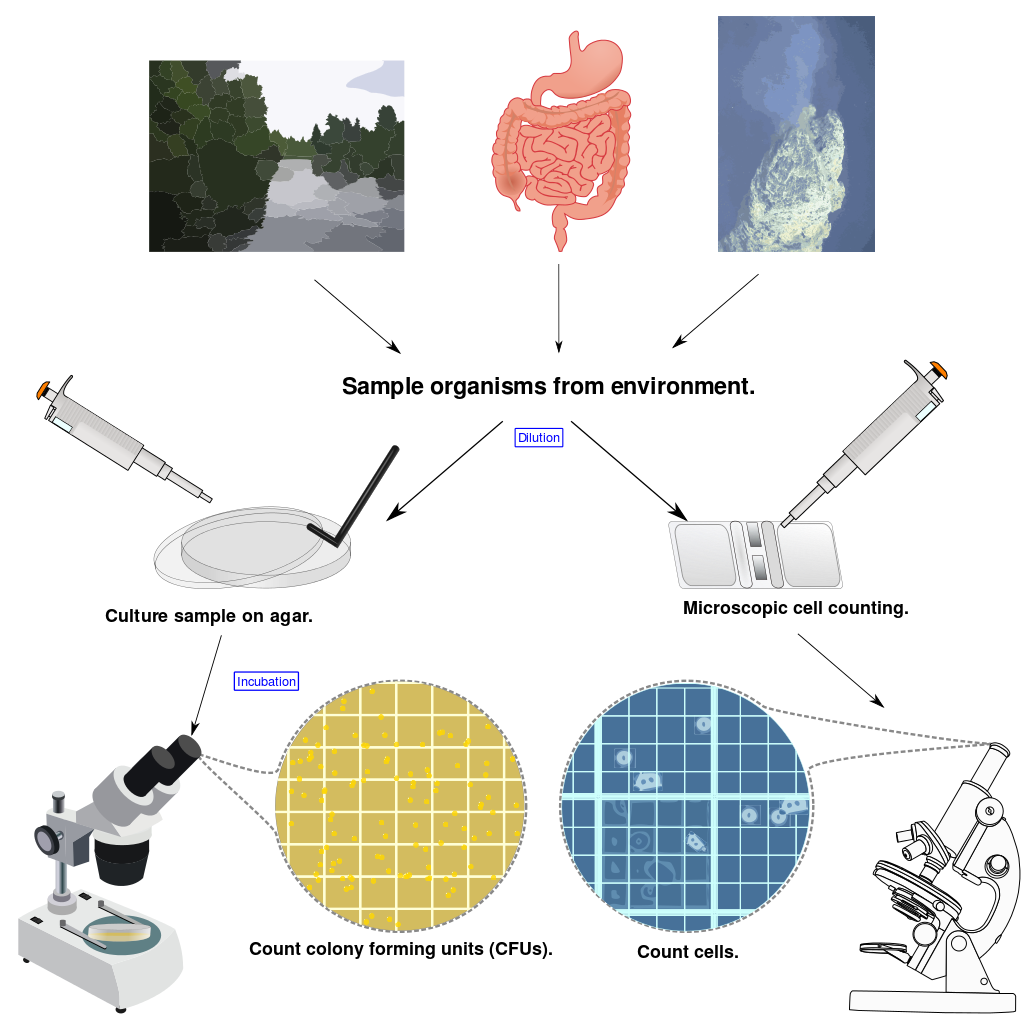
\includegraphics[width=\textwidth]{./images/Great-plate-count-anomaly}
			\end{center}
		\end{column}
		
		\begin{column}{0.5\textwidth}
			\begin{overlayarea}{0.9\textwidth}{0.9\textheight}
			\vspace{1mm}				
			\small{%
				\only<1->{%
				\begin{center}
					Counts of cells obtained via cultivation are orders of magnitude lower than those directly observed via microscope \cite{staley1985measurement}
				\end{center}}%
				\only<2->{%
				\begin{alertblock}{}				
				\begin{center}
					Using standard laboratory techniques, microbiologists are able to cultivate only 1\% of existent bacteria \cite{hugenholtz2002exploring}				
				\end{center}					
				\end{alertblock}}%				
			}%
			\begin{center}			
				\only<3->{
\includegraphics[width=0.9\textwidth]{./images/metagenomics}}
			\end{center}
			\end{overlayarea}
		\end{column}
		
	\end{columns}
\end{frame}
%%%%%%%%%%%%%%%%%%%%%%%%%%%%%%%%%%%%%%%%%%%%%%%%%%%%%%%%%%%%%%%%%%%%%%%%%%%%%%%%%%%%%%%%%%%%%%%%%%%%%%%%%%%%%%%%%%%%%%%%%%%%%%%%%%%
%%% END - Slide 3
%%%%%%%%%%%%%%%%%%%%%%%%%%%%%%%%%%%%%%%%%%%%%%%%%%%%%%%%%%%%%%%%%%%%%%%%%%%%%%%%%%%%%%%%%%%%%%%%%%%%%%%%%%%%%%%%%%%%%%%%%%%%%%%%%%%

%%%%%%%%%%%%%%%%%%%%%%%%%%%%%%%%%%%%%%%%%%%%%%%%%%%%%%%%%%%%%%%%%%%%%%%%%%%%%%%%%%%%%%%%%%%%%%%%%%%%%%%%%%%%%%%%%%%%%%%%%%%%%%%%%%%
%%% START- Slide 4
%%%%%%%%%%%%%%%%%%%%%%%%%%%%%%%%%%%%%%%%%%%%%%%%%%%%%%%%%%%%%%%%%%%%%%%%%%%%%%%%%%%%%%%%%%%%%%%%%%%%%%%%%%%%%%%%%%%%%%%%%%%%%%%%%%%
\begin{frame}
	\begin{overlayarea}{\textwidth}{0.95\textheight}
		\only<1>{%
			\begin{center}
				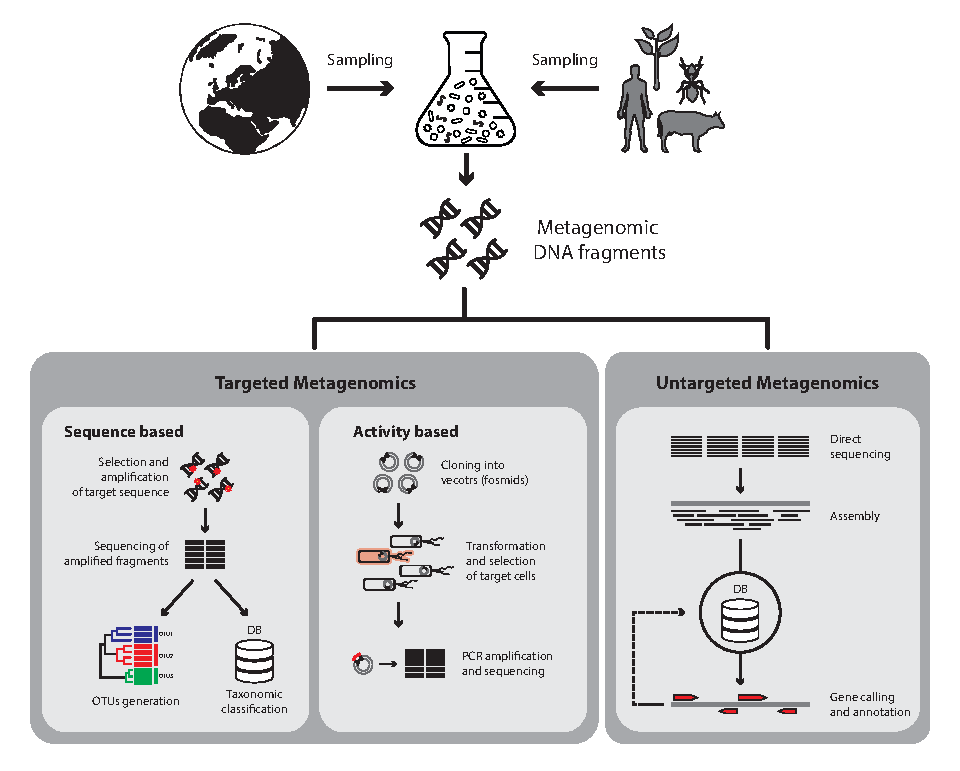
\includegraphics[width=0.93\textwidth]{./images/uber_pipeline_01}
			\end{center}}%
		\only<2>{%
			\begin{center}
				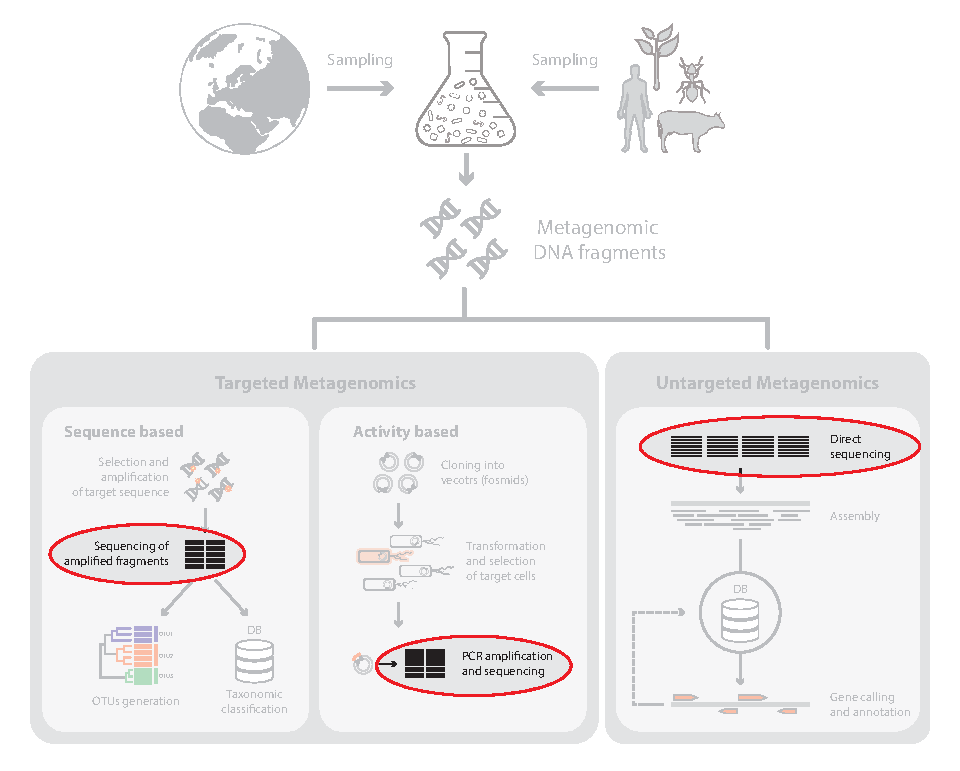
\includegraphics[width=0.93\textwidth]{./images/uber_pipeline_02}
				\vspace{-5cm}
				\begin{columns}
					\begin{column}{0.3\textwidth}
					% Nothing here
					\end{column}
					\begin{column}{0.3\textwidth}
						\begin{center}						
						\begin{alertblock}{}
						\begin{center}
							All approaches are based on high throughput sequencing technologies					
						\end{center}					
						\end{alertblock}
						\end{center}
					\end{column}	
					\begin{column}{0.4\textwidth}
					% Nothing here
					\end{column}
				\end{columns}			
			\end{center}}%	
	\end{overlayarea}		
\end{frame}
%%%%%%%%%%%%%%%%%%%%%%%%%%%%%%%%%%%%%%%%%%%%%%%%%%%%%%%%%%%%%%%%%%%%%%%%%%%%%%%%%%%%%%%%%%%%%%%%%%%%%%%%%%%%%%%%%%%%%%%%%%%%%%%%%%%
%%% END - Slide 4
%%%%%%%%%%%%%%%%%%%%%%%%%%%%%%%%%%%%%%%%%%%%%%%%%%%%%%%%%%%%%%%%%%%%%%%%%%%%%%%%%%%%%%%%%%%%%%%%%%%%%%%%%%%%%%%%%%%%%%%%%%%%%%%%%%%

%%%%%%%%%%%%%%%%%%%%%%%%%%%%%%%%%%%%%%%%%%%%%%%%%%%%%%%%%%%%%%%%%%%%%%%%%%%%%%%%%%%%%%%%%%%%%%%%%%%%%%%%%%%%%%%%%%%%%%%%%%%%%%%%%%%
%%% START - Slide 5
%%%%%%%%%%%%%%%%%%%%%%%%%%%%%%%%%%%%%%%%%%%%%%%%%%%%%%%%%%%%%%%%%%%%%%%%%%%%%%%%%%%%%%%%%%%%%%%%%%%%%%%%%%%%%%%%%%%%%%%%%%%%%%%%%%%
\begin{frame}
	\vspace{-6mm}
	\begin{overlayarea}{\textwidth}{\textheight}
	\begin{block}{DNA sequencing timeline}
	\begin{center}
	%\large\textbf{{DNA sequencing timeline}}
	\scriptsize{
	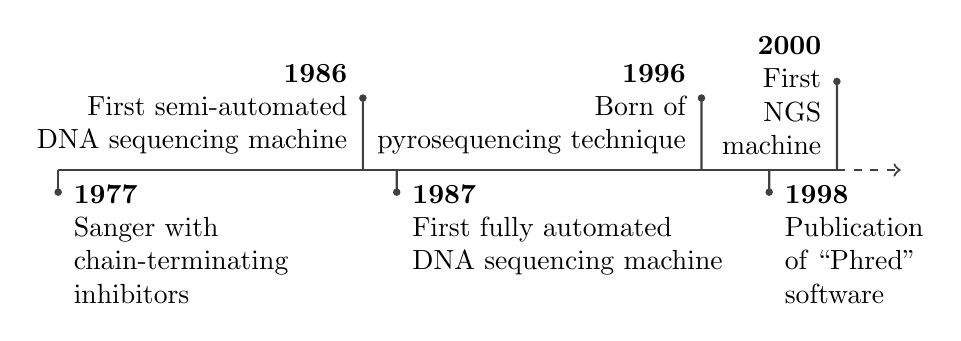
\begin{tikzpicture}
	
		% Vertical lines (all the same)
		%\foreach \x in {0, 3.87, 4.30, 8.17, 9.03, 9.89}
		%\draw [darkgray, thick] (\x cm,3pt) -- (\x cm,-3pt);
		
		% Vertical lines all different
		% 1977 - 0x down
		\draw [darkgray, thick] (0,0) -- (0cm,-8pt);
		\draw [darkgray, fill] (0cm, -8pt) circle [radius=0.04];
		
		% 1986 - 3.87x up
		\draw [darkgray, thick] (3.87,0) -- (3.87cm, 26pt);
		\draw [darkgray, fill] (3.87cm, 26pt) circle [radius=0.04];
		
		% 1987 - 4.30x down
		\draw [darkgray, thick] (4.30,0) -- (4.30cm,-8pt);
		\draw [darkgray, fill] (4.30cm, -8pt) circle [radius=0.04];
		
		% 1996 - 8.17x up
		\draw [darkgray, thick] (8.17,0) -- (8.17cm, 26pt);
		\draw [darkgray, fill] (8.17cm, 26pt) circle [radius=0.04];
		
		% 1998 - 9.03x down
		\draw [darkgray, thick] (9.03,0) -- (9.03cm,-8pt);
		\draw [darkgray, fill] (9.03cm, -8pt) circle [radius=0.04];
		
		% 2000 - 9.89x up
		\draw [darkgray, thick] (9.89,0) -- (9.89cm, 32pt);
		\draw [darkgray, fill] (9.89cm, 32pt) circle [radius=0.04];
		
		% Labels		
		\draw (0,0) node[below right=3pt, align=left] {\textbf{1977}\\Sanger with\\chain-terminating\\inhibitors};
		\draw (3.87,0) node[above left=3pt, align=right] {\textbf{1986}\\First semi-automated\\DNA sequencing machine};
		\draw (4.30,0) node[below right=3pt, align=left] {\textbf{1987}\\First fully automated\\DNA sequencing machine};
		\draw (8.17,0) node[above left=3pt, align=right] {\textbf{1996}\\Born of\\pyrosequencing technique};
		\draw (9.03,0) node[below right=3pt, align=left] {\textbf{1998}\\Publication\\of ``Phred''\\software};
		\draw (9.89,0) node[above left=3pt, align=right] {\textbf{2000}\\First\\NGS\\machine};
				
		% Horizontal timeline			
		\draw  [darkgray, thick] (0,0) -- (9.89,0);
		\draw  [->] [darkgray, dashed, thick] (9.89,0) -- (10.7,0);
	\end{tikzpicture}	
	}
	\end{center}
	\tiny{\hfill{\cite{sanger1977dna, smith1986fluorescence, prober1987system, ronaghi1996real, ewing1998base, brenner2000gene}}}
	\end{block}
	%
	\pause
	\scriptsize{%
	\only<2>{%
	\begin{columns}
		\begin{column}{0.6\textwidth}\\
			\tiny{%
			\begin{tikzpicture}
				\draw (0,5) node[inner sep=0]{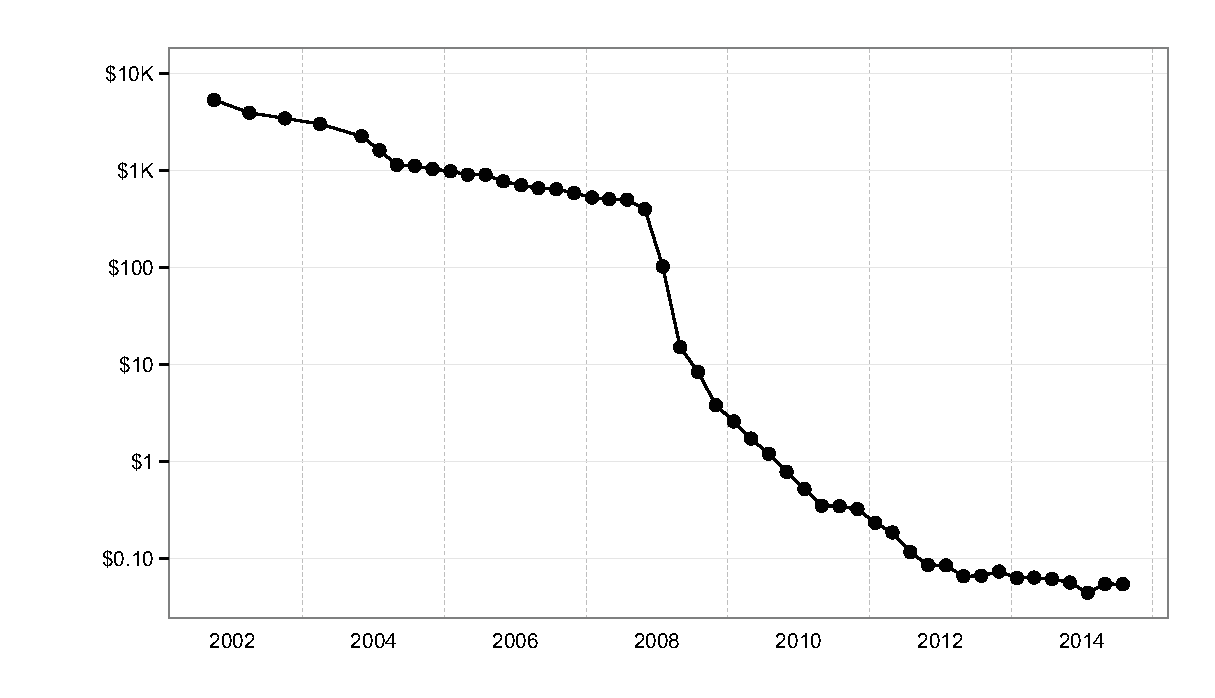
\includegraphics[width=\textwidth]{./images/seq_cost}};
				\draw (0.2,5) node[above=1.6cm, align=center]{\scriptsize{Average cost for raw megabase of DNA sequence}};
				
				% Pyrosequencing
			    \draw (-1.4,3.52) -- (-1.4,4.5);
			    \draw [fill] (-1.4,4.5) circle [radius=0.03];
			    \draw (-1.4,4.5) node[right=1pt, align=left] {454\\pyrosequencing};
			    
    				% Illumina
			    \draw (-1.1,3.52) -- (-1.1,4);
			    \draw [fill] (-1.1,4) circle [radius=0.03];
			    \draw (-1.1,4) node[right=1pt, align=left] {Illumina};
			    
     			% SOLiD
			    \draw (0.2,3.52) -- (0.2,4);
			    \draw [fill] (0.2,4) circle [radius=0.03];
			    \draw (0.2,4) node[right=1pt, align=left] {SOLiD};
			    
        			% Ion Torrent
			    \draw (1.3,3.52) -- (1.3,5);
			    \draw [fill] (1.3,5) circle [radius=0.03];
			    \draw (1.3,5) node[left=1pt, align=right] {Ion\\Torrent};
			    
			 	% PacBio
			    \draw (2.2,3.52) -- (2.2,4.3);
			    \draw [fill] (2.2,4.3) circle [radius=0.03];
			    \draw (2.2,4.3) node[left=1pt, align=right] {PacBio};			    
			\end{tikzpicture}
			}%
		\end{column}
		%
		\begin{column}{0.4\textwidth}
			\normalsize{%
			With the development of new technologies the cost for sequencing one megabase of DNA has been reduced by more than 1000 times
			}
		\end{column}		
	\end{columns}	
	}
	\only<3>{%
	\begin{columns}
		\begin{column}{0.6\textwidth}
			\begin{center}
				\begin{tikzpicture}
				\draw (0,5.5) node[inner sep=0]{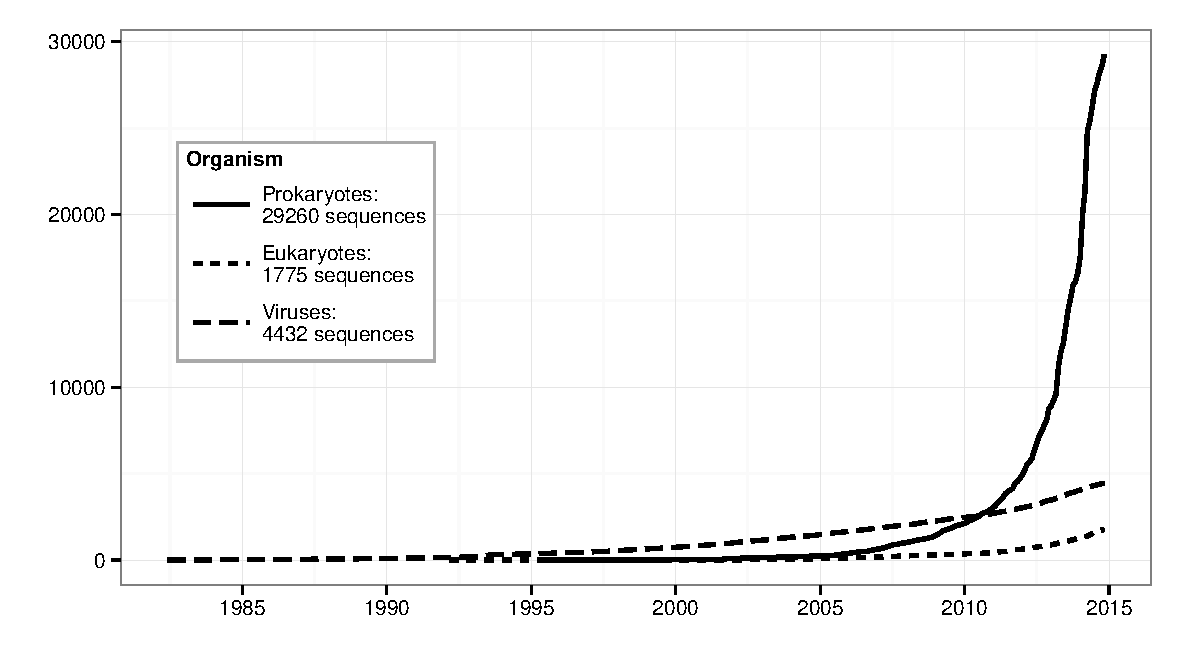
\includegraphics[width=0.9\textwidth]{./images/seq_number_genebank}};
				\draw (0.2,5.5) node[above=1.5cm, align=center]{Number of genome sequences submitted to Genbank};
				
				% NGS era
				\draw (1,4.25) -- (1,6);
				\draw [fill] (1,6) circle [radius=0.03];
				\draw (1,6) node[above=1pt, align=center] {NGS era};
				\end{tikzpicture}	
			\end{center}
		\end{column}
		%
		\begin{column}{0.4\textwidth}
			\normalsize{%
			The ``NGS era'' has lead to a drastic increment of genome sequences available in public databases
			}	
		\end{column}		
	\end{columns}
	}
	}
	\end{overlayarea}
\end{frame}
%%%%%%%%%%%%%%%%%%%%%%%%%%%%%%%%%%%%%%%%%%%%%%%%%%%%%%%%%%%%%%%%%%%%%%%%%%%%%%%%%%%%%%%%%%%%%%%%%%%%%%%%%%%%%%%%%%%%%%%%%%%%%%%%%%%
%%% END - Slide 5
%%%%%%%%%%%%%%%%%%%%%%%%%%%%%%%%%%%%%%%%%%%%%%%%%%%%%%%%%%%%%%%%%%%%%%%%%%%%%%%%%%%%%%%%%%%%%%%%%%%%%%%%%%%%%%%%%%%%%%%%%%%%%%%%%%%

%%%%%%%%%%%%%%%%%%%%%%%%%%%%%%%%%%%%%%%%%%%%%%%%%%%%%%%%%%%%%%%%%%%%%%%%%%%%%%%%%%%%%%%%%%%%%%%%%%%%%%%%%%%%%%%%%%%%%%%%%%%%%%%%%%%
%%% START - Slide 6
%%%%%%%%%%%%%%%%%%%%%%%%%%%%%%%%%%%%%%%%%%%%%%%%%%%%%%%%%%%%%%%%%%%%%%%%%%%%%%%%%%%%%%%%%%%%%%%%%%%%%%%%%%%%%%%%%%%%%%%%%%%%%%%%%%%
\begin{frame}
	\tikzstyle{era} = [text=black, rectangle, draw, fill=blue!20, text width=1.8cm, text centered, rounded corners, minimum height=0.8cm]
	\tikzstyle{bad} = [text=black, rectangle, draw, fill=red!20, text width=4cm, text centered, rounded corners, minimum height=1cm]
	\tikzstyle{good} = [text=black, rectangle, draw, fill=green!20, text width=4cm, text centered, rounded corners, minimum height=1cm]
	\tikzstyle{normal} = [black, text=black, rectangle, draw, fill=white, rounded corners]
	\tikzstyle{problems} = [black, text=black, rectangle, draw, fill=black!10, rounded corners]	
	\tikzstyle{line} = [draw, -latex']
	
\begin{overlayarea}{\textwidth}{0.9\textheight}	
\begin{tikzpicture}[node distance = 0.3cm, auto]
	\scriptsize{%
	\only<1->{%
    % Place nodes
    \node [era] (NGS) {\normalsize{\textbf{NGS Era}}};
    \node [good, below right=of NGS, align=left] (disciplines) {%
    		\parbox{4cm}{%
			\begin{itemize}
			    \item Born of Metagenomics
			    \item Improvements in Genomics 
			\end{itemize}%
		}
	};
    \node [bad, below left=of NGS, align=left] (problems) {%
	    \parbox{4cm}{%
			\begin{itemize}
			    \item Huge amount of data
			    \item Less human control 
			\end{itemize}%
		}
    	};    	
    	% Draw edges
    \path [line] (NGS) to [out=0, in=90] (disciplines);
    \path [line] (NGS) to [out=180, in=90] (problems);
    	}
    	\only<2->{%
	% Other two nodes    	
    	\node [problems, below=1cm of problems, align=left, node distance=2cm] (metprob){%
    		\textbf{Tecnical Problems:}\\
    		\parbox{4cm}{%
			\begin{itemize}
			    \item[*] Handling huge data			    
			    \item[*] Mining databases
			    \item[*] Control of generated data
			    \item[*] Lack of dedicated tools
			\end{itemize}%
		}
    	};
    	
    	\node [problems, below right=1cm and 1cm of problems, align=left, node distance=2cm] (bioprob){%
    		\textbf{Biological Problems:}\\
    		\parbox{4cm}{%
			\begin{itemize}
			    \item[*] Difficult interpretation			    
			    \item[*] Hard visualization
			    \item[*] Selection of significant data
			    \item[*] Lack of standard methods
			\end{itemize}%
		}
    	};
    
    % Other edges
    \path [line] (problems) to [out=270, in=90] (metprob);
    \path [line] (problems) to [out=275, in=90] (bioprob);
    }
    
    \only<3->{%
    	% Other two nodes    	
    	\node [normal, below=0.8cm of metprob, align=left, node distance=2cm] (bigtool){%
    		\textbf{Small tool for Big data:}\\
    		\parbox{4cm}{% 	
		\begin{itemize}
			\item[\checkmark] Raw data control
			\item[\checkmark] Tools evaluation
		\end{itemize}
    		}
    	};
    	
    	\node [normal, right=0.6cm of bigtool, align=left, node distance=2cm] (bactenv){%
    		\parbox[t]{2.8cm}{%
    			\textbf{Bacterial world:}\\
    			\vspace{-2.5mm}
    			\begin{itemize}
    				\item[\checkmark] Bacteria in the environment    				
    			\end{itemize}
		}
		\parbox[t]{2.8cm}{%
			\textbf{Bacterial landlord:}\\
			\vspace{-2.5mm}
			\begin{itemize}
				\item[\checkmark] Bacterial symbiosis
				\item[\checkmark] Bacterial infections
			\end{itemize}
		}
    	};
    
    % Other edges
    \path [line] (metprob) to [out=270, in=90] (bigtool);
    \path [line] (bioprob) to [out=270, in=90] (bactenv);
    }
    }
\end{tikzpicture}
\end{overlayarea}
\end{frame}
%%%%%%%%%%%%%%%%%%%%%%%%%%%%%%%%%%%%%%%%%%%%%%%%%%%%%%%%%%%%%%%%%%%%%%%%%%%%%%%%%%%%%%%%%%%%%%%%%%%%%%%%%%%%%%%%%%%%%%%%%%%%%%%%%%%
%%% END - Slide 6
%%%%%%%%%%%%%%%%%%%%%%%%%%%%%%%%%%%%%%%%%%%%%%%%%%%%%%%%%%%%%%%%%%%%%%%%%%%%%%%%%%%%%%%%%%%%%%%%%%%%%%%%%%%%%%%%%%%%%%%%%%%%%%%%%%%
%%%%%%%%%%%%%%%%%%%%%%%%%%%%%%%%%%%%%%%%%%%%%%%%%%%%%%%%%%%%%%%%%%%%%%%%%%%%%%%%%%%%%%%%%%%%%%%%%%%%%%%%%%%%%%%%%%%%%%%%%%%%%%%%%%%
%%% END - BACKGROUND
%%%%%%%%%%%%%%%%%%%%%%%%%%%%%%%%%%%%%%%%%%%%%%%%%%%%%%%%%%%%%%%%%%%%%%%%%%%%%%%%%%%%%%%%%%%%%%%%%%%%%%%%%%%%%%%%%%%%%%%%%%%%%%%%%%%


%%%%%%%%%%%%%%%%%%%%%%%%%%%%%%%%%%%%%%%%%%%%%%%%%%%%%%%%%%%%%%%%%%%%%%%%%%%%%%%%%%%%%%%%%%%%%%%%%%%%%%%%%%%%%%%%%%%%%%%%%%%%%%%%%%%
%%% START - SMALL TOOLS FOR BIG DATA
%%%%%%%%%%%%%%%%%%%%%%%%%%%%%%%%%%%%%%%%%%%%%%%%%%%%%%%%%%%%%%%%%%%%%%%%%%%%%%%%%%%%%%%%%%%%%%%%%%%%%%%%%%%%%%%%%%%%%%%%%%%%%%%%%%%
\section{Small tools for big data}
\subsection{}

%%%%%%%%%%%%%%%%%%%%%%%%%%%%%%%%%%%%%%%%%%%%%%%%%%%%%%%%%%%%%%%%%%%%%%%%%%%%%%%%%%%%%%%%%%%%%%%%%%%%%%%%%%%%%%%%%%%%%%%%%%%%%%%%%%%
%%% START - Slide 7
%%%%%%%%%%%%%%%%%%%%%%%%%%%%%%%%%%%%%%%%%%%%%%%%%%%%%%%%%%%%%%%%%%%%%%%%%%%%%%%%%%%%%%%%%%%%%%%%%%%%%%%%%%%%%%%%%%%%%%%%%%%%%%%%%%%
%\begin{frame}
%	\tikzstyle{line} = [draw,thick, -latex']
%	\begin{overlayarea}{\textwidth}{0.9\textheight}
%	\begin{center}
%	
%	\begin{tikzpicture}[node distance = 0.3cm, auto]
%		\only<1->{%
%		\node [inner sep=0] (before) {\includegraphics[width=0.4\textwidth]{./images/per_base_quality_before}};
%		\node [inner sep=0, right=2cm of before, align=left] (after) {\parbox{4cm}{%
%			There is a drop of quality passing from the first bases of the sequence to the last ones due to pre-phasing and post-phasing erros}};	
%		}
%		\only<2->{%
%		\node [inner sep=0, right=2cm of before] (after) {\includegraphics[width=0.4\textwidth]{./images/per_base_quality_after}};		
%		\path [line] (before) -> (after);
%		}		
%	\end{tikzpicture}
%	\end{center}
%	\end{overlayarea}
%\end{frame}

\begin{frame}
	\textbf{\Large{DNA sequencing control}}
	\begin{columns}
		\begin{column}{0.7\textwidth}
			Chromatogram:
			\includegraphics[width=\textwidth]{./images/dna_sequence.png}		
		\end{column}
		\begin{column}{0.3\textwidth}
			Quality:
			\includegraphics[width=\textwidth]{./images/per_base_quality_before}
		\end{column}		
	\end{columns}
	\begin{columns}
		\begin{column}{0.35\textwidth}
			\begin{align*}
				Q &= Quality\\
				P &= Error Probability\\
				\\
				Q &= -10 \, \log_{10} P\\
				P &= 10^{-^{Q}/_{10}}\\
			\end{align*}		
		\end{column}
		\begin{column}{0.65\textwidth}
			\only<1>{%
			\begin{block}{}
				A quality value $Q$ is an integer representing the probability that the corresponding base call is incorrect ($P$).\\
				Wrong bases may lead to the production of incorrect data.
			\end{block}
			}
			\only<2>{%
				
\includegraphics[width=0.8\textwidth]{./images/Dont_panic}
			}
		\end{column}		
	\end{columns}
\end{frame}
%%%%%%%%%%%%%%%%%%%%%%%%%%%%%%%%%%%%%%%%%%%%%%%%%%%%%%%%%%%%%%%%%%%%%%%%%%%%%%%%%%%%%%%%%%%%%%%%%%%%%%%%%%%%%%%%%%%%%%%%%%%%%%%%%%%
%%% END - Slide 7
%%%%%%%%%%%%%%%%%%%%%%%%%%%%%%%%%%%%%%%%%%%%%%%%%%%%%%%%%%%%%%%%%%%%%%%%%%%%%%%%%%%%%%%%%%%%%%%%%%%%%%%%%%%%%%%%%%%%%%%%%%%%%%%%%%%

%%%%%%%%%%%%%%%%%%%%%%%%%%%%%%%%%%%%%%%%%%%%%%%%%%%%%%%%%%%%%%%%%%%%%%%%%%%%%%%%%%%%%%%%%%%%%%%%%%%%%%%%%%%%%%%%%%%%%%%%%%%%%%%%%%%
%%% START - Slide 8
%%%%%%%%%%%%%%%%%%%%%%%%%%%%%%%%%%%%%%%%%%%%%%%%%%%%%%%%%%%%%%%%%%%%%%%%%%%%%%%%%%%%%%%%%%%%%%%%%%%%%%%%%%%%%%%%%%%%%%%%%%%%%%%%%%%
\begin{frame}
	\begin{tikzpicture}
		\node (text) {\textbf{\Large{StreamingTrim 1.0}}};
		\node [inner sep=0, right=2.2cm of text.south ,anchor=south west, align=left] (logo) {\includegraphics[width=0.56\textwidth]{./images/streamingtrim}};
	\end{tikzpicture}
	\vspace{5mm}
	\begin{columns}
		\begin{column}{0.5\textwidth}
			\begin{center}
				Dynamic Window Algorithm\\
				\vspace{2mm}
				\includegraphics[width=\textwidth]{./images/dynamic_pipeline_all}			
			\end{center}			
		\end{column}
		\begin{column}{0.5\textwidth}
			\only<2->{%
				\begin{tikzpicture}
					\node [inner sep=0] (zscore) {\includegraphics[width=\textwidth]{./images/zscore}};
					\node [draw=black, fill=white, below=0.3cm of zscore, rounded corners] (frm) {\tiny{%
					$Z_{score} = \log_{10} \bigg( \frac{Quality\:improvement}{Length\:decrease} \bigg)$}};
				\end{tikzpicture}
				\vspace{-8mm}
			}
		\end{column}			
	\end{columns}
\end{frame}
%%%%%%%%%%%%%%%%%%%%%%%%%%%%%%%%%%%%%%%%%%%%%%%%%%%%%%%%%%%%%%%%%%%%%%%%%%%%%%%%%%%%%%%%%%%%%%%%%%%%%%%%%%%%%%%%%%%%%%%%%%%%%%%%%%%
%%% END - Slide 8
%%%%%%%%%%%%%%%%%%%%%%%%%%%%%%%%%%%%%%%%%%%%%%%%%%%%%%%%%%%%%%%%%%%%%%%%%%%%%%%%%%%%%%%%%%%%%%%%%%%%%%%%%%%%%%%%%%%%%%%%%%%%%%%%%%%

%%%%%%%%%%%%%%%%%%%%%%%%%%%%%%%%%%%%%%%%%%%%%%%%%%%%%%%%%%%%%%%%%%%%%%%%%%%%%%%%%%%%%%%%%%%%%%%%%%%%%%%%%%%%%%%%%%%%%%%%%%%%%%%%%%%
%%% START - Slide 9
%%%%%%%%%%%%%%%%%%%%%%%%%%%%%%%%%%%%%%%%%%%%%%%%%%%%%%%%%%%%%%%%%%%%%%%%%%%%%%%%%%%%%%%%%%%%%%%%%%%%%%%%%%%%%%%%%%%%%%%%%%%%%%%%%%%
\begin{frame}
	\begin{overlayarea}{\textwidth}{0.99\textheight}
	\begin{block}{RDP Classifier}
		\small{\textit{The RDP Classifier is a naive Bayesian classifier which was developed to provide rapid taxonomic placement based on rRNA sequence data. The RDP Classifier can rapidly and accurately classify bacterial and archaeal 16s rRNA sequences, and Fungal LSU sequences. It provides taxonomic assignments from domain to genus, with confidence estimates for each assignment.}\\
		\hfill{[RDP staff]}}
	\end{block}
	\begin{columns}
		\begin{column}{0.5\textwidth}
			\includegraphics[width=0.8\textwidth]{./images/rdp_percentages}	
		\end{column}
		\begin{column}{0.5\textwidth}
			\only<2>{%
				\includegraphics[width=0.9\textwidth]{./images/all_rdp}	
			}
			\only<3>{%
				\includegraphics[width=\textwidth]{./images/genus_rdp}
			}
		\end{column}		
	\end{columns}
	\end{overlayarea}
\end{frame}
%%%%%%%%%%%%%%%%%%%%%%%%%%%%%%%%%%%%%%%%%%%%%%%%%%%%%%%%%%%%%%%%%%%%%%%%%%%%%%%%%%%%%%%%%%%%%%%%%%%%%%%%%%%%%%%%%%%%%%%%%%%%%%%%%%%
%%% END - Slide 9
%%%%%%%%%%%%%%%%%%%%%%%%%%%%%%%%%%%%%%%%%%%%%%%%%%%%%%%%%%%%%%%%%%%%%%%%%%%%%%%%%%%%%%%%%%%%%%%%%%%%%%%%%%%%%%%%%%%%%%%%%%%%%%%%%%%

\section{References}
\subsection{}
\begin{frame}[allowframebreaks] 
	\tiny
	\bibliography{References}
\end{frame}

\end{document}